% The contents of this file is
% Copyright (c) 2009-  Charles R. Severance, All Righs Reserved

\chapter{Tradutores Voluntários}


\section*{Eduardo Cândido}

Eduardo Fernando Barboza Candido é MESTRE EM ENGENHARIA DE COMPUTAÇÃO - Engenharia de Software, pelo IPT-SP (2015), Pós-Graduado em Banco de Dados e Análise de Sistemas e Tecnólogo em processamentos de Dados pela Escola de Engenharia de Lins. Atua com análise/desenvolvimento de sistemas e Administração de Banco de Dados (DBA) a mais de 25 anos. Possui certificaçao OCP 9i - Oracle. Teve o interesse por Python despertado durante um projeto de automatização de compra e venda de ações na BOVESPA (em andamento) em conjunto com Victor Jabur que lhe apresentou a linguagem. Contagiado com o entusiasmo em ajudar aos outros demonstrado pelo Victor, decidiu participar da tradução deste livro, contribuindo, então, com a tradução do capítulo 2. Atualmente tem se dedicado a estudar os caminhos que levam a formação de Cientistas de Dados.

\begin{description}
\itemsep0em 
\item[E-mail] efbcandido@yahoo.com.br
\end{description}

\beforefig
\centerline{\includegraphics[height=1.50in]{translators/eduardobarboza.eps}}
\afterfig

\newpage

\section*{Felipe Nogueira Souza}

Felipe Nogueira de Souza, marido da Dani, pai do Lucas, da Anna e do Pedro. Possui mais de 8 anos de experiência em eletrônica e TI. Tecnólogo em Informática para Gestão de Negócios pela FATEC, Faculdade de Tecnologia do Estado de São Paulo e atualmente cursando bacharelado em Sistemas de Informação na UFSCAR, Universidade Federal de São Carlos. Tem estudado Python há cerca de 3 anos com foco em Desenvolvimento Web e Data Science (Machine Learning).

\begin{description}
\itemsep0em 
\item[Website] http://fnscoder.com
\item[GitHub] https://github.com/fnscoder
\end{description}

\beforefig
\centerline{\includegraphics[height=1.50in]{translators/felipesouza.eps}}
\afterfig

\section*{Fernando José Moreira}

Fernando José Moreira é um profissional com 10 anos de experiência na área de informática. Formado em Tecnologia em Processamento de Dados pela - UNIVALE MBA em Engenharia de Software Orientada a Serviços pela - FIAP Amplo conhecimento da arquitetura e solução técnica para carga e migração de dados utilizando o Oracle da Integrator. Elaboração e construção de integrações utilizando SOA, Integrações com Sistemas Legados utilizando BPEL e OSB.

\begin{description}
\itemsep0em 
\item[LinkedIn] https://www.linkedin.com/in/fernandojosemoreira
\end{description}

\beforefig
\centerline{\includegraphics[height=1.50in]{translators/fernandojosemoreira.eps}}
\afterfig

\newpage

\section*{Herbert Parentes Fortes Neto}

Herbert Parentes Fortes Neto é Bacharel em Psicologia e também atuou no mercado de ações. É Desenvolvedor Debian, contribuindo com empacotamento, sendo membro dos times de multimídia, de ferramentas de fotografia, QA (Quality Assurance) e também do time de tradução. Atualmente está estudando Python.

\begin{description}
\itemsep0em 
\item[GitHub] https://github.com/hpfn/
\end{description}

\beforefig
\centerline{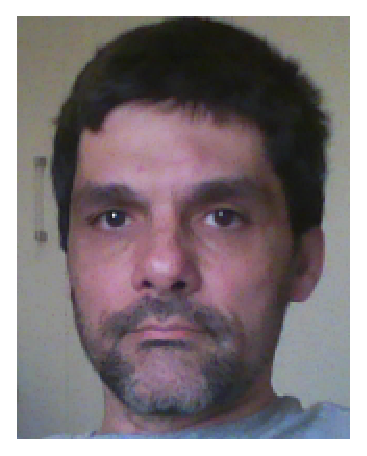
\includegraphics[height=1.50in]{translators/herbertfortes.eps}}
\afterfig

\section*{João Vitor S. de Sousa}

João Vitor S. de Sousa é estudante de Sistemas de Informação na Universidade de Mogi das Cruzes, entusiasta por desenvolvimento de software desde os 11 anos, quando conheceu o Blender. Atualmente desenvolve serviços web utilizando Python e JavaScript .

\begin{description}
\itemsep0em 
\item[E-mail] joao_vitor_silvestre@outlook.com
\end{description}

\beforefig
\centerline{\includegraphics[height=2.00in]{translators/joaovitorsilvestre.eps}}
\afterfig

\newpage

\section*{Maykon Chagas}

Maykon Chagas é estudante eterno de Python. Simpatizante de Software Livre (FLOSS) não é desenvolvedor mas está sempre criando scripts em Python para ajudar na vida de administração de sistemas, até se perder na montueira arquivos .py. Entrou no projeto de tradução com o objetivo de ler o livro e ajudar outras pessoas a ter acesso ao material de ótima qualidade preparado pelo professor Charles Severance. Estudante, pesquisador e agora buscando um emprego ou algo que me dê sustento. Deseja mudar o mundo com códigos e dispositivos livres, mas já fica feliz quando consegue fazer os seus amigos que isso é um direito da sociedade, e não só um pensamento paranóico subversivo.

\begin{description}
\itemsep0em 
\item[Twitter] https://twitter.com/mchagas
\end{description}

\beforefig
\centerline{\includegraphics[height=1.50in]{translators/maykonchagas.eps}}
\afterfig

\section*{Paulo Henrique Silva}

Paulo Henrique da Silva, corredor amador, pai do Pedro e da Sarah, dedica-se ao estudo e desenvolvimento de software desde 2009, conheceu Python à pouco mais de 2 anos e vem desde então tendo uma relação cada vez mais forte com a linguagem, relação esta que foi aprimorada quando realizou o curso Programming for Everybody desenvolvido pela University of Michigan e ministrado pelo professor Charles Severance, formado em Ciência da Computação e atualmente cursando especialização em Qualidade e Engenharia de Software na UNIVALI, Paulo é sócio e gerente de projetos na empresa Catarina Touch.
 
\begin{description}
\itemsep0em 
\item[LinkedIn] https://br.linkedin.com/in/paulohesilva
\end{description}

\beforefig
\centerline{\includegraphics[height=1.50in]{translators/paulohesilva.eps}}
\afterfig

\newpage

\section*{Rafael Costa}

Rafael Costa, formado em Gestão de TI, mas sempre atuou como Sysadmin. Se aproximou do desenvolvimento através do Python e atualmente utiliza Python para as mais diversas tarefas de administração de sistemas. Agradecido por existirem iniciativas como a criação deste livro e sua tradução, são atitudes como estas que ajudam a disseminar o conhecimento.

\begin{description}
\itemsep0em 
\item[E-mail] phs.paulohenriquesilva@gmail.com
\end{description}

\section*{Rafael Covre}

Rafael Covre é Bacharel em Ciências Biológicas pela Universidade Federal de São Carlos (campus Sorocaba) e mestre em Bioinformática pela Universidade Federal do Paraná. Adora a natureza, tecnologia, programação e estatística. Acredita que um mundo melhor e mais justo é feito com mais Python e mais Open Source.

\beforefig
\centerline{\includegraphics[height=1.50in]{translators/rafaelcovre.eps}}
\afterfig

\newpage

\section*{Victor Jabur}

Victor Jabur é Bacharel em Sistemas de Informação pela Universidade de São Paulo (USP), atua com arquitetura e desenvolvimento de software
em diversas empresas brasileiras. Apaixonado por Python, amor à primeira vista, devido à facilidade de aprendizado, legibilidade de código,
comunidade ativa super empolgante, sempre ajudando uns aos outros. Atuou como coordenador / colaborador deste trabalho de tradução, graças
à autorização do professor Charles Severance, autor deste livro e toda a sua vontade de ajudar o próximo por meio da computação. Obrigado time, este trabalho só foi possível através da união, trabalho em equipe, comunicação e vontade de fazer deste mundo um lugar melhor. Plantamos nossa semente ! 

\begin{description}
\itemsep0em 
\item[LinkedIn] https://www.linkedin.com/in/victorjabur
\item[Blog] http://victorjabur.com
\item[GitHub] https://github.com/victorjabur
\end{description}

\beforefig
\centerline{\includegraphics[height=1.50in]{translators/victorjabur.eps}}
\afterfig


\clearemptydoublepage

% TABLE OF CONTENTS
\begin{latexonly}

\tableofcontents

\clearemptydoublepage

\end{latexonly}

% START THE BOOK
\mainmatter